\section{Introduction}

\label{sec:introduction}

\subsection{Task and Motivation}

A knowledge graph (KG) stores facts as nodes and edges. Graph repair has
two linked decisions: which errors to fix and which rules to get. A repair
needs a rule that can detect its target error. Getting a rule has a cost.
Its value depends on the errors that remain. A scheduler uses the current
graph and rules to choose the next action.

Experts supply rules for known needs. Source text can supply further rules
about entity types, hierarchies, and required steps. Large language models
(LLMs) can propose these rules. We check the rule format, vocabulary, and
matched records before using a proposal to detect errors.

We use reinforcement learning (RL) to divide a fixed budget between graph
and rule actions. We also use two prompts to generate rules from text.
An active rule changes which repairs are available. A repair changes which
rules the graph needs next.

We test this link in three stages. First, a fixed rule library supports
comparisons of learned policies, simple schedules, and rewards. Second,
saved paired responses show what deletion and augmentation each generate.
Third, direct rule execution and document tests show which candidates
lead to repairs. The first stage trains policies. The third stage uses
fixed schedules.

\subsection{Contributions}

We make three contributions:
\begin{enumerate}
    \item \textbf{A graph--rule control environment.} Fourteen input
    features describe the graph, rules, and budget. Eight actions change
    graph records or active rules. An action mask lists the allowed choices.
    The reward includes quality gains and action costs.
    \item \textbf{A Double-DQN policy and shared-condition tests.}
    Temporary duplicates explain why the count penalty blocks relation
    repair. Forty neural models and ten one-step fitted baselines compare
    three penalties. Component tests measure graph features, rule features,
    action masking, and call cost. The rate penalty improves repair, and
    the action mask raises final F1.
    \item \textbf{Two rule-generation prompts and source-linked tests.}
    Deletion and augmentation share an output format. Equal-call tests
    measure candidate counts. Execution logs link each type pattern to
    its original response. Fixed schedules and document tests measure
    repairs, correct facts kept, and the effect of rule order.
\end{enumerate}

Figure~\ref{fig:rl_framework} shows the method. The policy receives
fourteen features for graph quality, rule quality, remaining errors,
remaining budget, and active rule shares. The action mask lists allowed
actions. After each action, the environment updates quality and reward.
Separate action tests inspect graph changes from saved states.

\begin{figure*}[t]
    \centering
    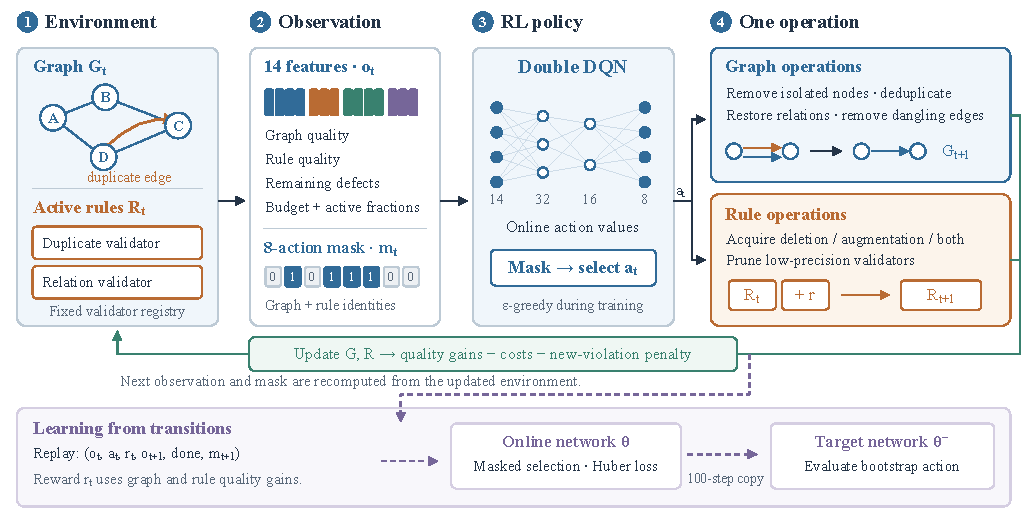
\includegraphics[width=0.96\textwidth]{figure/method/cooptimization.pdf}
    \caption{Learning graph and rule actions. The environment gives fourteen inputs and a mask of eight actions. The policy chooses one action. The environment updates quality and reward. The lower band shows Double-DQN replay training. Small graphs and mask entries show example states. The loop uses a fixed rule library. Figure~\ref{fig:dual_strategy} gives the text prompts.}
    \label{fig:rl_framework}
\end{figure*}

\subsection{Paper Outline}

Section~\ref{sec:related_work} reviews earlier work.
Section~\ref{sec:methodology} gives the scheduling model and rule prompts.
Section~\ref{sec:experiments} gives the three test stages and discussion.
The appendices give protocols, execution logs, and further repair tests.
